\documentclass[11pt]{article}

\usepackage[margin=1in]{geometry}
\usepackage{amsmath,amssymb}
\usepackage{booktabs}
\usepackage{graphicx}
\usepackage{microtype}
\usepackage{float}
\usepackage{caption}
\usepackage{subcaption}
\usepackage{xcolor}
\usepackage[hidelinks]{hyperref}
\usepackage{enumitem}
\usepackage{array}

\graphicspath{{../artifacts/}}
\setlength{\parskip}{0.45em}
\setlength{\parindent}{0pt}
\setlist{nosep}
\captionsetup{font=small}

\newcommand{\code}[1]{\texttt{#1}}
\newcommand{\E}{\mathbb{E}}
\newcommand{\Prb}{\mathop{\mathrm{Pr}}}
\newcommand{\Normal}{\mathcal{N}}

\title{Methods and Simulation Results for Bayesian Inference from Repeated Size Profiles}
\author{}
\date{\today}

\begin{document}
\maketitle

\section{Methods}

\subsection{Inferential targets}

The simulation study distinguished four inferential targets:
\begin{enumerate}
  \item individual-level survival, growth, and reproductive output as
  functions of individual size;
  \item population-effective transition rates after averaging over unobserved
  attributes and demographic stochasticity;
  \item functionals of the fitted projection kernel, including the dominant
  eigenvalue; and
  \item prediction of future size profiles.
\end{enumerate}
The individual-level vital rates were the primary targets for recovery
experiments. This distinction was necessary because a model may accurately
predict profile dynamics while estimating a population-effective transition
operator that differs from the individual generating rates.

\subsection{Individual-based population generator}

At census time \(t\), individual \(i\) had size \(x_{it}\), age \(a_{it}\),
sex \(q_i\), and optional persistent latent quality \(u_i\). Survival was
generated as an individual Bernoulli event,
\begin{equation}
  S_{it} \sim \operatorname{Bernoulli}
  \left\{s(x_{it},a_{it},q_i,u_i,E_t,N_t)\right\},
\end{equation}
where \(E_t\) denotes an environmental covariate and \(N_t\) denotes
population size. Conditional on survival, next-census size was generated from
a normal growth distribution,
\begin{equation}
  x_{i,t+1}\mid S_{it}=1
  \sim \Normal\left\{m_g(x_{it},a_{it},q_i,u_i,E_t,N_t),
  \sigma_g^2(x_{it},a_{it},q_i,u_i,E_t,N_t)\right\}.
\end{equation}
The number of realized recruits entering the next census was generated
separately,
\begin{align}
  R_{it} &\sim \operatorname{Poisson}
  \left\{r(x_{it},a_{it},q_i,u_i,E_t,N_t)\right\},\\
  x_{\mathrm{recruit},t+1} &\sim
  \Normal\left\{m_b(x_{it},E_t),\sigma_b^2\right\}.
\end{align}
Survival, growth, and reproduction were therefore separate stochastic
individual events. The simulated population did not evolve by deterministic
application of the recovery IPM.

For the initial broad experiments, the generating rates were
\begin{align}
  \operatorname{logit}\{s(x)\} &= -2.2 + 0.032x,\\
  m_g(x) &= \max(x,\,x+18-0.12x), \qquad \sigma_g=4.5,\\
  r_i(x) &= I(q_i=\mathrm{female})\exp(-7+0.075x),\\
  m_b(x) &= 43+0.02x, \qquad \sigma_b=3.5.
\end{align}
The corresponding population-average recruitment rate incorporated the
one-half expected female proportion. In later multi-truth experiments, the
generator was parameterized directly from the recovery-model coefficients,
with female reproductive output doubled so that its population average
matched the declared recruitment curve.

\subsection{Size-profile observation process}

Individual identities were retained by the generator but discarded before
profile-only analysis. At each census, individuals were independently sampled
with profile detection probability \(q_t(x)\), optionally with size
measurement error. Observed sizes were grouped into equally spaced bins with
centers \(x_j\), width \(\Delta x\), and bounds
\((\ell_j,u_j]\). The baseline experiments used 5-mm bins.

The general observation intensity was
\begin{equation}
  \lambda_t(x)=e_tq_t(x)\mu_t(x),
\end{equation}
where \(\mu_t(x)\) is latent population intensity and \(e_t\) is survey effort.
Most experiments used known constant effort and size-independent detection.
Conditional on the initial observed profile, subsequent bin counts were
modeled using either
\begin{equation}
  Y_{tj}\sim\operatorname{Poisson}(M_{tj})
\end{equation}
or a Gamma--Poisson model,
\begin{align}
  \Lambda_{tj}\mid M_{tj},\phi
    &\sim\operatorname{Gamma}(\phi,\phi/M_{tj}),\\
  Y_{tj}\mid\Lambda_{tj}
    &\sim\operatorname{Poisson}(\Lambda_{tj}),
\end{align}
which yields a negative-binomial marginal distribution with mean \(M_{tj}\)
and precision \(\phi\).

\subsection{Positive inverse IPM}

The recovery model propagated latent size intensity through a decomposed
kernel,
\begin{align}
  \mu_{t+1}(x') &= \int K(x',x)\mu_t(x)\,dx,\\
  K(x',x) &= P(x',x)+F(x',x),\\
  P(x',x) &= s(x)g(x'\mid x),\\
  F(x',x) &= r(x)b(x'\mid x).
\end{align}
The conditional growth and recruit-size densities were normalized:
\begin{equation}
  \int g(x'\mid x)\,dx'=1,\qquad
  \int b(x'\mid x)\,dx'=1.
\end{equation}
Consequently, column integrals of \(P\) and \(F\) corresponded to survival and
recruitment intensity. This normalization removed arbitrary scaling within
each component, although it did not guarantee identification of the
decomposition of \(K\) into \(P\) and \(F\).

Vital-rate coefficients were centered at 80 mm, with
\(z(x)=(x-80)/20\):
\begin{align}
  \operatorname{logit}\{s(x)\}
    &= \alpha_s+\beta_sz(x),\\
  m_g(x)-x
    &= \max\{0,\alpha_g+\beta_gz(x)\},\\
  \sigma_g &= \exp(\eta_g),\\
  \log r(x)
    &= \alpha_r+\beta_rz(x),\\
  m_b(x)
    &= \alpha_b+\beta_bz(x),\\
  \sigma_b &= \exp(\eta_b).
\end{align}
The baseline model therefore estimated ten demographic coefficients.

\subsection{Numerical integration}

The continuous operator was discretized on a regular size mesh:
\begin{equation}
  \boldsymbol{\mu}_{t+1}
  = \Delta x\,\mathbf{K}\boldsymbol{\mu}_t.
\end{equation}
All kernel elements and projected intensities remained nonnegative.
Conditional normal transition probabilities were integrated over target-size
bins,
\begin{equation}
  \Prb(\ell_j<X'\leq u_j\mid x)
  =
  \Phi\left\{\frac{u_j-m(x)}{\sigma}\right\}
  -
  \Phi\left\{\frac{\ell_j-m(x)}{\sigma}\right\},
\end{equation}
rather than evaluating normal densities only at bin centers. The resulting
bin probabilities were normalized over the retained mesh. This correction was
important when the 5-mm bins were wide relative to recruit-size variation.

\subsection{Prior distributions}

The broad Monte Carlo study used independent weakly informative normal priors
on transformed coefficients. Selected induced 95\% prior intervals were
approximately:
\begin{center}
\begin{tabular}{lcc}
\toprule
Quantity & Prior median & Approximate 95\% interval\\
\midrule
Survival at 80 mm & 0.60 & 0.07--0.97\\
Growth increment at 80 mm & 8.0 & 0--19.8 mm\\
Growth SD & 5.0 & 1.3--19.6 mm\\
Recruitment at 80 mm & 0.20 & 0.01--3.78\\
Recruit mean size at 80 mm & 45.0 & 25.5--64.6 mm\\
Recruit-size SD & 4.0 & 1.0--15.8 mm\\
\bottomrule
\end{tabular}
\end{center}
These priors were diffuse on biologically meaningful scales but retained
structural information through the logistic and log links, parametric curve
forms, normalized transition distributions, and nonnegative growth
constraint. The Gamma--Poisson process precision received
\(\log\phi\sim\Normal\{\log(50),2^2\}\).

\subsection{External fecundity information}

Auxiliary information was represented as an independent fecundity study. For
an external study of \(n_e\) fish, standardized parent sizes \(z_i\) were
balanced from \(-1.5\) to \(1.5\), and realized offspring counts were
generated as
\begin{equation}
  C_i\sim\operatorname{Poisson}
  \left[\exp\{\alpha_r^{(e)}+\beta_r^{(e)}z_i\}\right].
\end{equation}
The external study was analyzed using a Poisson regression with the diffuse
fecundity prior. A bivariate normal Laplace approximation to its posterior,
including covariance between recruitment level and slope, became the
external-study prior for the profile analysis.

Under full borrowing, this external posterior directly replaced the diffuse
prior for \((\alpha_r,\beta_r)\). Under robust borrowing, the prior was
\begin{equation}
  \pi_{\mathrm{robust}}(\alpha_r,\beta_r)
  =
  w\,\pi_e(\alpha_r,\beta_r)
  +(1-w)\,\pi_0(\alpha_r,\beta_r),
  \qquad w=0.8,
\end{equation}
where \(\pi_e\) denotes the external-study posterior approximation and
\(\pi_0\) denotes the diffuse fecundity prior.

Because the robust posterior could be genuinely multimodal, it was not
approximated by a single Gaussian mode. Separate Laplace approximations were
fitted under the external and diffuse components. Their posterior component
weights were estimated from Laplace marginal-evidence approximations, and
posterior draws were sampled from the resulting two-component mixture.

\subsection{Posterior computation and approximation audit}

Broad simulation grids used maximum a posteriori optimization and Gaussian
Laplace posterior approximations. Non-positive-definite posterior Hessians
were retained as approximation-failure records and excluded from scientific
coverage summaries. Six representative datasets were also fitted using four
adaptive-Metropolis chains. Across this audit, the median absolute difference
between Laplace and MCMC posterior means was 0.106 MCMC posterior standard
deviations, the median Laplace-to-MCMC posterior-SD ratio was 0.988, parameter
coverage agreement was 100\%, maximum split \(\widehat R\) was 1.063, and
minimum approximate effective sample size was 66.

\subsection{Simulation experiments}

\subsubsection{Broad design grid}

The first broad grid varied allocation of a fixed 12-transition budget,
initial population size, profile detection, initial size-profile shape, and
recovery likelihood (Table~\ref{tab:broad-grid}).

\begin{table}[H]
\centering
\caption{Factors in the broad Monte Carlo design.}
\label{tab:broad-grid}
\begin{tabular}{ll}
\toprule
Factor & Levels\\
\midrule
Transition design & \(1\times12,\ 3\times4,\ 6\times2\)\\
Initial population per trajectory & 500, 2500\\
Fraction observed per annual profile & 0.25, 1.00\\
Initial profile & baseline, small-fish cohort pulse\\
Independent replicates & 10\\
Recovery likelihood & Poisson, Gamma--Poisson\\
\bottomrule
\end{tabular}
\end{table}

This grid produced 240 independently simulated datasets and 480 Bayesian
fits. The fixed transition budget separated the benefit of longer
within-population follow-up from replication among independent population
trajectories.

\subsubsection{Auxiliary-fecundity experiment}

The targeted auxiliary experiment used the \(3\times4\) design, an initial
population of 500 fish, and 25\% profile detection. Thirty fresh profile
datasets were independently generated. Each was analyzed using profiles
alone; correctly transportable external fecundity studies of 50, 200, or 800
fish; an 800-fish biased external study with full borrowing; and an 800-fish
biased external study with robust borrowing. Analyses were paired within
profile dataset.

\subsubsection{Transportability-boundary experiment}

The transportability experiment considered three biological truths: baseline
rates; survival at 80 mm reduced from 0.589 to 0.400; and recruitment slope per
20 mm reduced from 1.50 to 0.60. For each truth, ten fresh \(3\times4\)
profile datasets were generated. Each dataset was paired with an 800-fish
external fecundity study.

Transport bias jointly shifted external-study recruitment level and slope:
\begin{align}
  \alpha_r^{(e)} &= \alpha_r + 0.50d,\\
  \beta_r^{(e)} &= \beta_r - 0.30d,
\end{align}
where \(d\in\{0,0.25,0.50,0.75,1.00,1.50\}\). At \(d=0.25\), the external
recruitment curve was approximately 27\% higher at 50 mm, 13\% higher at
80 mm, and 1\% higher at 110 mm. Profiles-only, full-borrowing, and
robust-borrowing analyses were compared on the same simulated datasets.

\subsubsection{Paired profile and individual-data benchmark}

The paired-data benchmark generated 200 independent datasets, each containing
three populations with four annual transitions, 500 initial fish per
population, 25\% profile detection, and 35\% known capture probability. Six
analyses were fitted to each dataset: Poisson profiles only, Gamma--Poisson
profiles only, capture--recapture transitions only, Poisson integrated
profiles and capture--recapture, Gamma--Poisson integrated profiles and
capture--recapture, and a complete-history oracle.

Conditional on capture of individual \(i\) in year \(t\), consecutive
recapture was modeled as
\begin{equation}
  C_{i,t+1}\mid C_{it}=1,x_{it}
  \sim \operatorname{Bernoulli}\{s(x_{it})q\},
\end{equation}
where \(q=0.35\) was known. If recaptured, next-year size was modeled using
the same conditional growth distribution as the inverse IPM. These data
therefore informed survival and growth but supplied no reproductive or
parent--offspring information. The oracle observed every individual survival
outcome, growth transition, offspring count including zeros, parent--offspring
link, and recruit size.

\subsection{Performance measures}

Performance measures included posterior bias, root mean squared error (RMSE),
95\% interval width and coverage, and approximation diagnostics. Recruitment
curve RMSE was evaluated at 50, 80, and 110 mm. Auxiliary-study analyses were
compared with profiles-only analyses using paired RMSE ratios. Bootstrap
intervals resampled paired datasets. For the exploratory transportability
boundary, borrowing was called safe only when the 95\% bootstrap interval for
the paired RMSE ratio was below one and coverage did not fall below
profiles-only coverage.

\section{Simulation Results}

\subsection{Numerical integration and initial identifiability}

Evaluating conditional normal densities at 5-mm bin centers produced an
artificial recruit-variance bias when the true recruit-size SD was 3.5 mm.
Integrating normal probabilities over target bins removed this artifact.
Numerical construction of the kernel was therefore consequential for
inference rather than merely an implementation choice.

In the initial multi-year Bayesian experiment, repeated profiles accurately
recovered survival probabilities and recruit-size means over representative
sizes. With 12 transitions, estimated survival probabilities at 50, 80, and
110 mm were approximately 0.357, 0.589, and 0.787, compared with generating
values 0.354, 0.589, and 0.789. In contrast, recruitment level, recruitment
slope, some growth quantities, and the dominant eigenvalue were biased and
overconfident. Recruitment level and slope had posterior correlations near
\(-0.99\) in short series. Additional years increased precision but could
concentrate the posterior around a population-effective pseudo-truth that
differed from individual generating rates.

\subsection{Broad Monte Carlo recovery}

The broad grid completed without fit failures; 98.96\% of posterior Hessians
were positive definite. Five non-positive-definite Poisson approximations were
excluded from scientific coverage summaries.

\begin{table}[H]
\centering
\caption{Mean 95\% interval coverage by allocation of the 12-transition
budget.}
\label{tab:design-coverage}
\small
\setlength{\tabcolsep}{4pt}
\begin{tabular}{lcccc}
\toprule
Design & Poisson parameters & Poisson derived &
Gamma--Poisson parameters & Gamma--Poisson derived\\
\midrule
\(1\times12\) & 0.734 & 0.701 & 0.764 & 0.718\\
\(3\times4\)  & 0.795 & 0.775 & 0.818 & 0.818\\
\(6\times2\)  & 0.795 & 0.813 & 0.816 & 0.836\\
\bottomrule
\end{tabular}
\end{table}

Replicated trajectories outperformed one long trajectory on average
(Table~\ref{tab:design-coverage}). However, very short trajectories retained
recruitment-level/slope confounding. No design achieved nominal 95\%
coverage across all parameters and derived quantities.

\begin{figure}[H]
\centering
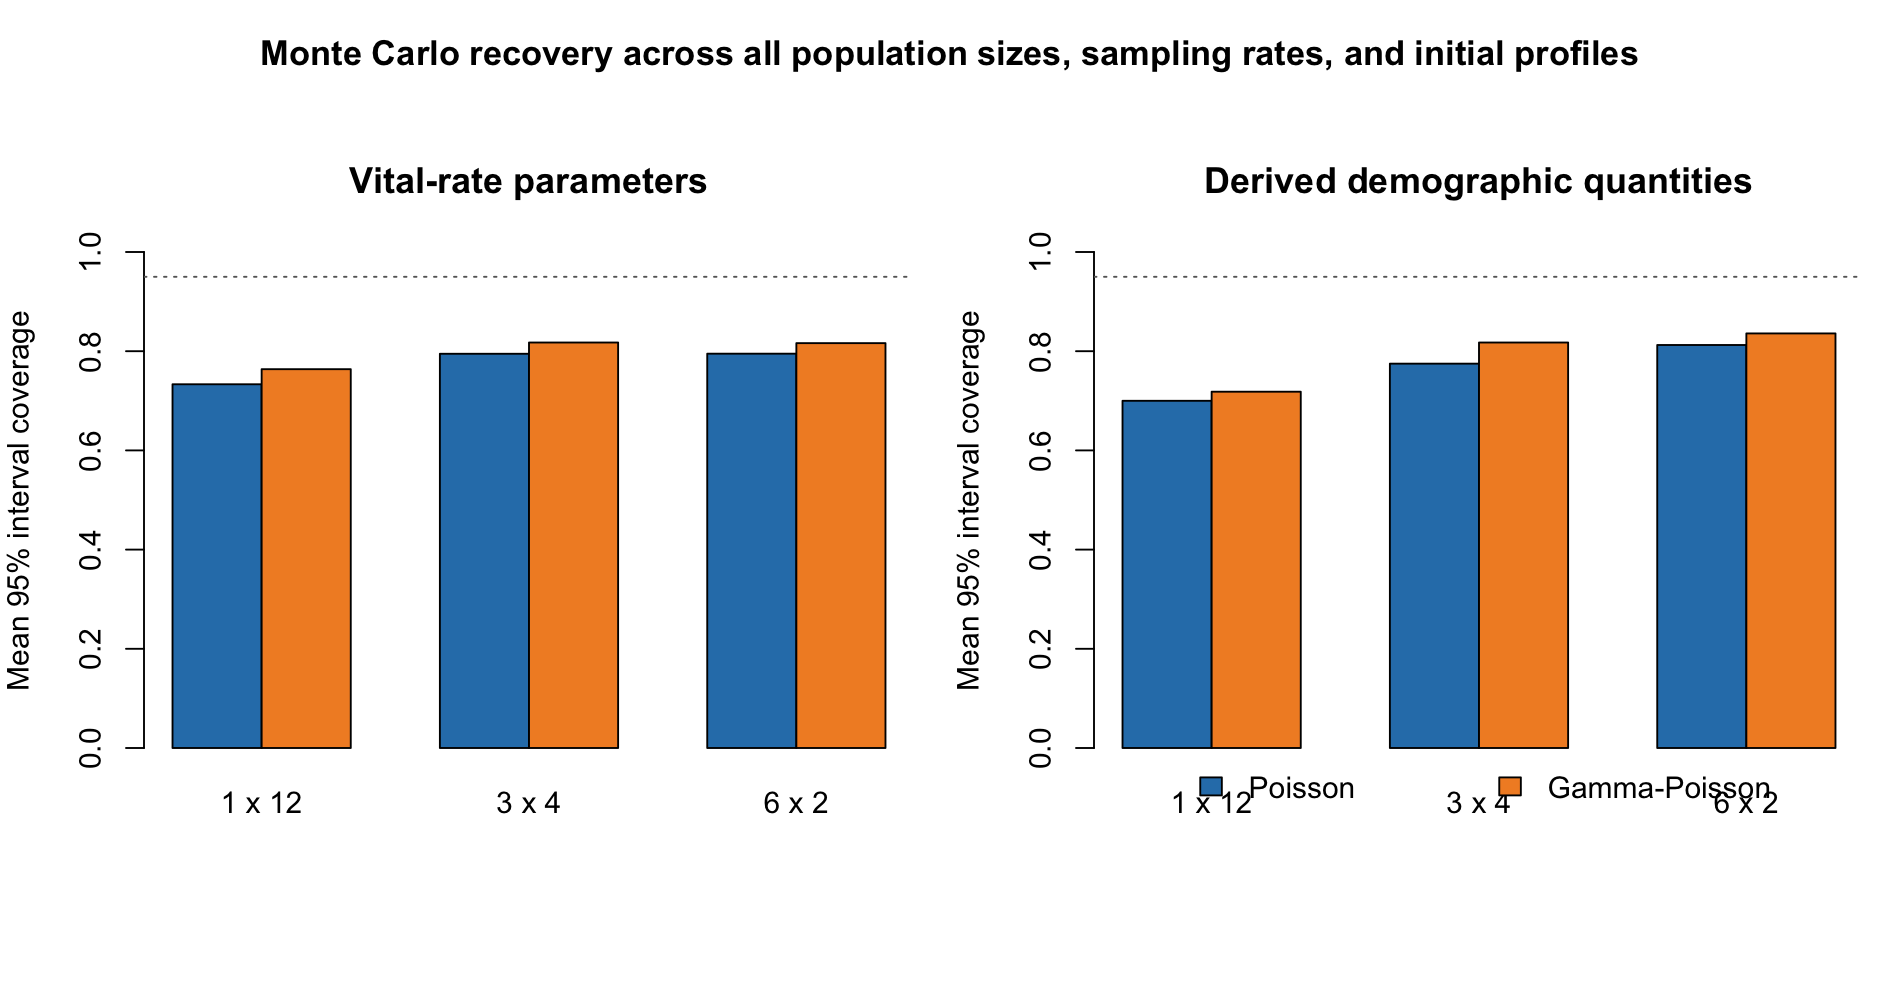
\includegraphics[width=0.92\textwidth]{monte_carlo/coverage_by_design.png}
\caption{Mean interval coverage across the broad simulation grid. Replicated
trajectories generally improved recovery relative to one long trajectory, but
coverage remained below nominal levels.}
\label{fig:coverage-design}
\end{figure}

Increasing population size and profile completeness provided only modest
improvement. Under Poisson recovery, mean parameter coverage increased from
0.755 for \(N=500\) with 25\% detection to 0.795 for \(N=2500\) with complete
profiles. The dominant limitation was decomposition of profile change into
demographic mechanisms rather than uncertainty about annual profile shapes.

\begin{table}[H]
\centering
\caption{Selected Gamma--Poisson coverage rates across the broad grid.}
\label{tab:quantity-coverage}
\begin{tabular}{lr}
\toprule
Quantity & Coverage\\
\midrule
Recruit-size SD & 0.958\\
Recruit mean at 110 mm & 0.929\\
Recruit mean at 80 mm & 0.908\\
Growth increment at 50 mm & 0.892\\
Survival at 50 mm & 0.879\\
Survival at 80 mm & 0.829\\
Growth SD & 0.754\\
Dominant eigenvalue & 0.617\\
Recruitment at 80 mm & 0.571\\
\bottomrule
\end{tabular}
\end{table}

The size distribution of recruits was recoverable, whereas recruitment
intensity was not (Table~\ref{tab:quantity-coverage} and
Figure~\ref{fig:quantity-coverage}). Independent Gamma--Poisson overdispersion
modestly improved average coverage but did not resolve the primary structural
confounding.

\begin{figure}[H]
\centering
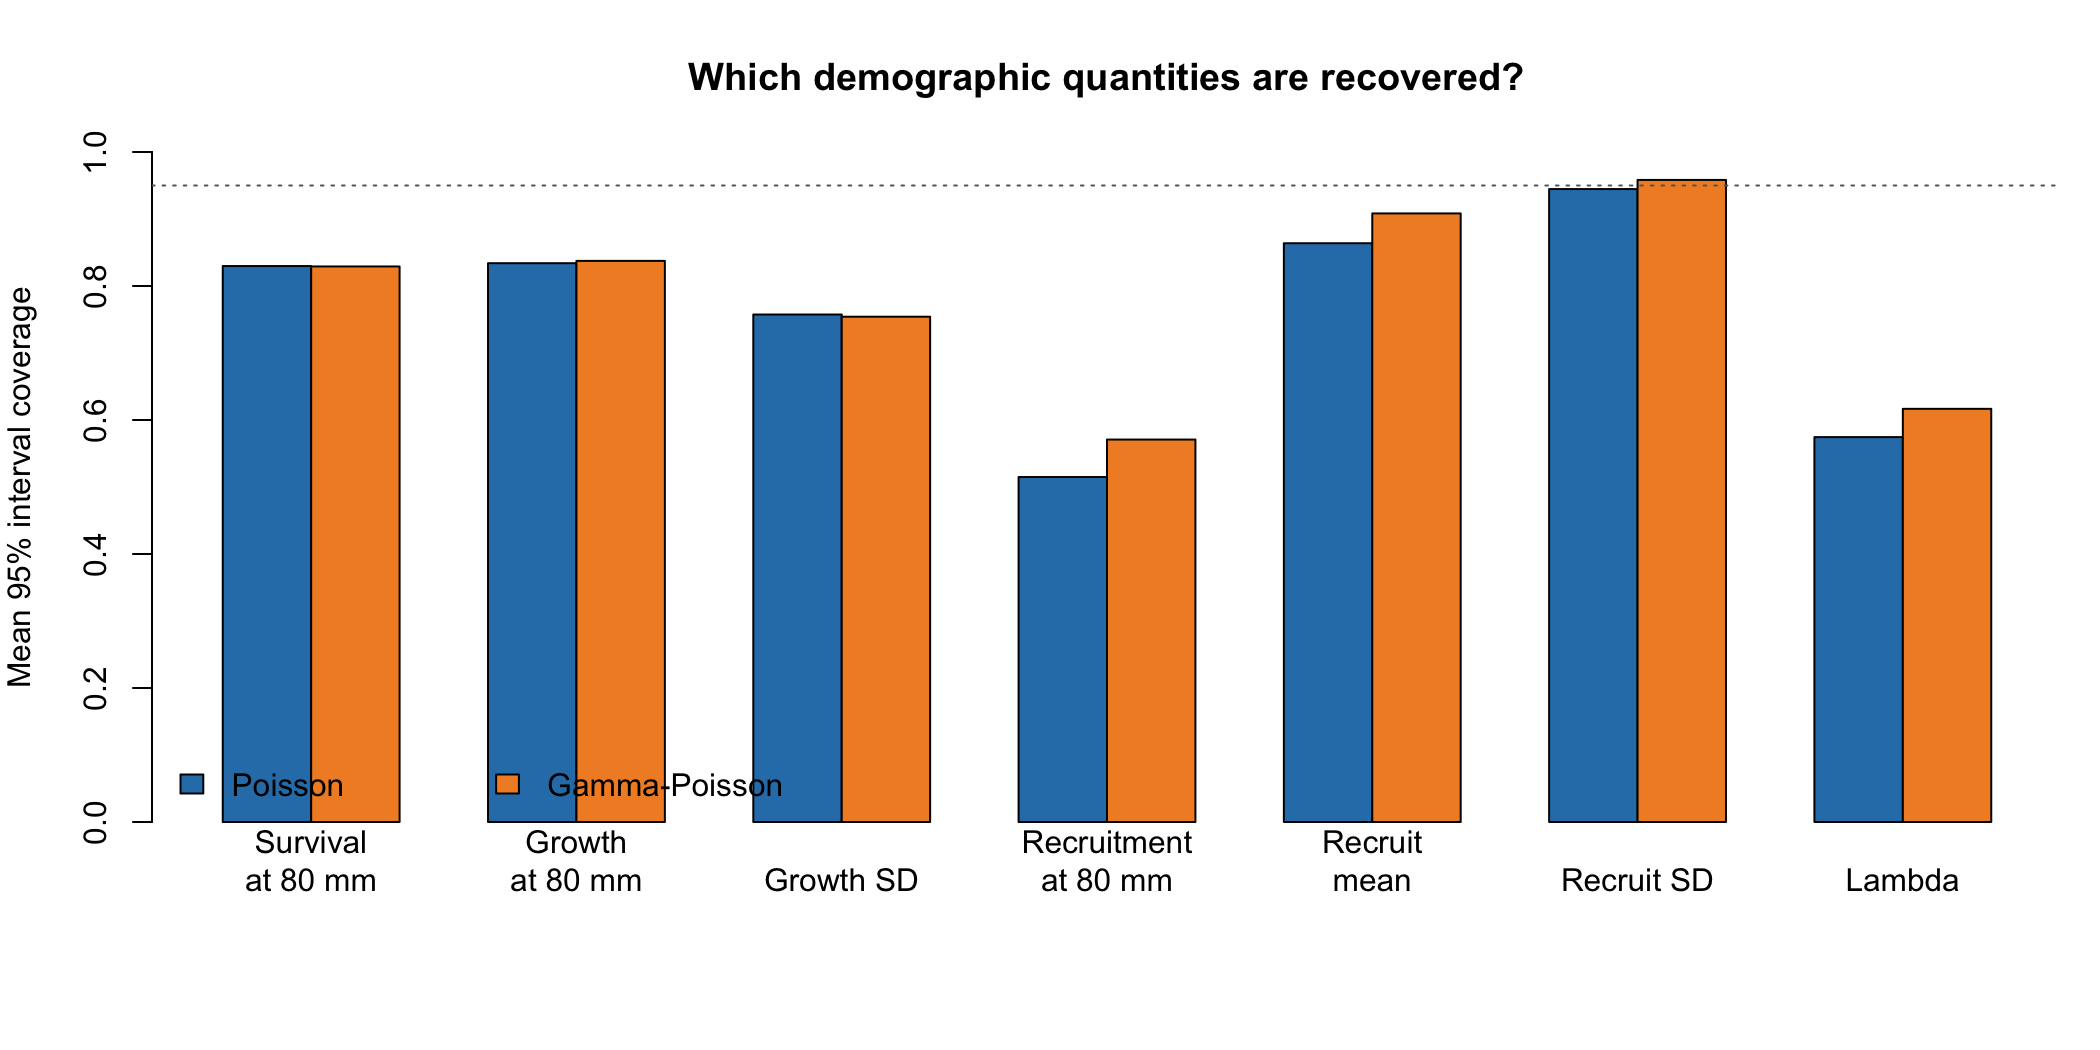
\includegraphics[width=0.92\textwidth]{monte_carlo/coverage_by_quantity.png}
\caption{Coverage varied substantially among demographic quantities.
Recruit-size distributions, survival, and mean growth were more reliably
recovered than recruitment intensity and the dominant eigenvalue.}
\label{fig:quantity-coverage}
\end{figure}

Applying the same small-fish cohort pulse to all populations did not uniformly
improve recovery and reduced coverage for the \(3\times4\) design. Useful
perturbations must distinguish competing demographic mechanisms rather than
simply add variation.

\subsection{Moderate prior information}

Moderately informative external priors, with uncertainty twice that of the
initial oracle priors, changed most posterior summaries only modestly. Across
the targeted prior-information experiment, mean coverage was 0.747 under
diffuse priors, 0.769 with survival and growth information, 0.742 with
fecundity information, and 0.747 with information on all vital rates. Mean
relative absolute error decreased from 0.179 under diffuse priors to 0.161
with fecundity information and 0.155 with information on all rates.

The concentrated profile likelihood frequently overwhelmed moderate external
information, including along directions where it targeted a
population-effective pseudo-truth. Prior information was most useful when it
directly constrained the confounded mechanism. Recruit-size information did
not identify recruitment intensity.

\subsection{Targeted auxiliary fecundity data}

The confirmatory auxiliary-data experiment completed 180 analyses with no fit
failures. Two non-positive-definite approximations from one difficult dataset
were excluded from corresponding biased-prior summaries.

\begin{table}[H]
\centering
\caption{Confirmatory auxiliary-fecundity results across 30 fresh profile
datasets.}
\label{tab:aux-confirm}
\small
\setlength{\tabcolsep}{4pt}
\begin{tabular}{lccc}
\toprule
Analysis & Recruitment-curve RMSE & RMSE ratio & Coverage at 80 mm\\
\midrule
Profiles only & 0.280 & 1.000 & 0.533\\
Correct study, 50 fish & 0.190 & 0.679 & 0.433\\
Correct study, 200 fish & 0.123 & 0.440 & 0.600\\
Correct study, 800 fish & 0.084 & 0.299 & 0.867\\
Biased study, 800 fish, full borrowing & 0.102 & 0.366 & 0.000\\
Biased study, 800 fish, robust borrowing & 0.238 & 0.852 & 0.276\\
\bottomrule
\end{tabular}
\end{table}

Correctly transportable auxiliary fecundity data improved recruitment
recovery as the external sample increased (Table~\ref{tab:aux-confirm}).
Two hundred external fish reduced mean recruitment-curve RMSE by more than
half. Eight hundred external fish reduced RMSE by approximately 70\% and
increased recruitment-at-80 coverage from 53\% to 87\%.

\begin{figure}[H]
\centering
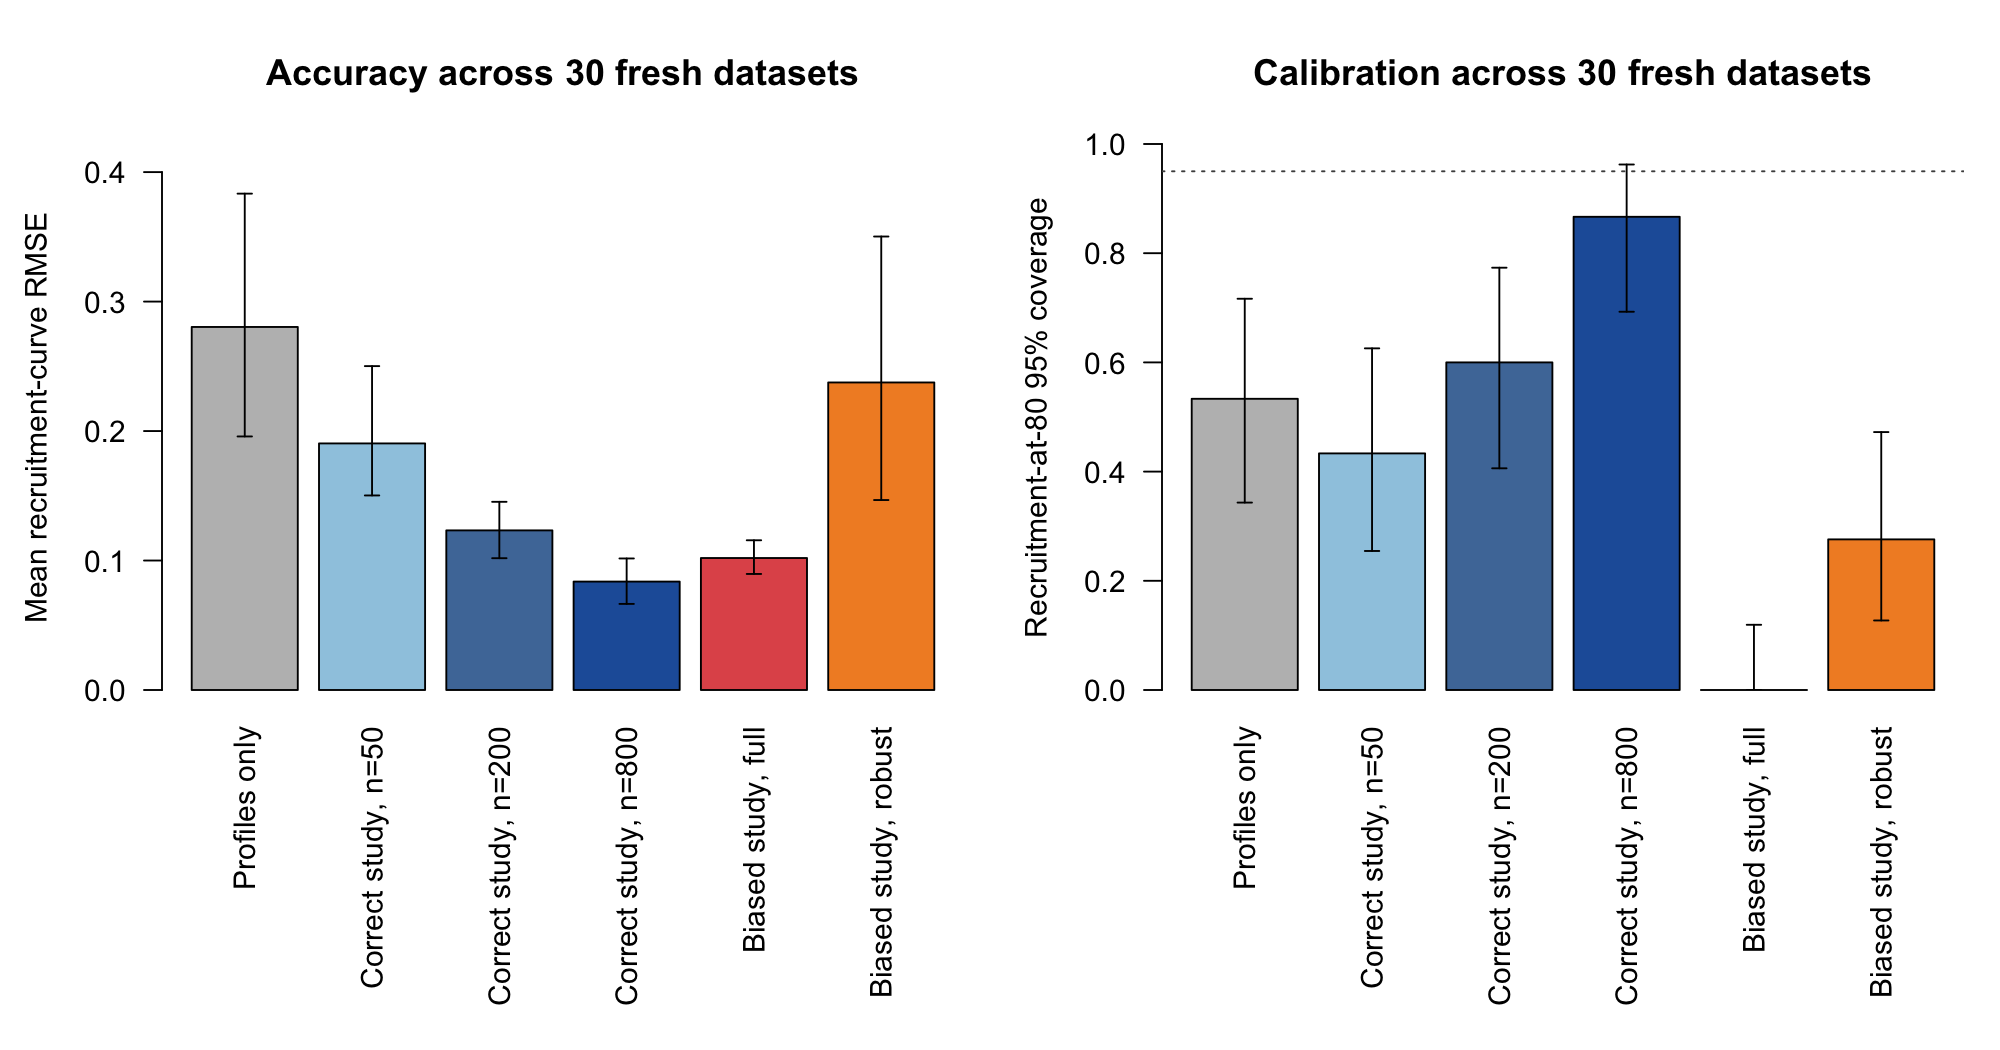
\includegraphics[width=\textwidth]{auxiliary_fecundity/confirmatory_results.png}
\caption{Confirmatory performance of targeted auxiliary fecundity data.
Correctly transportable external data improved accuracy and eventually
coverage. A precise biased study produced low RMSE but zero coverage; robust
borrowing reduced but did not eliminate the damage. Error bars are bootstrap
intervals for mean RMSE and exact binomial intervals for coverage.}
\label{fig:aux-confirm}
\end{figure}

The paired bootstrap 95\% intervals for RMSE ratios were 0.502--0.921 for 50
external fish, 0.306--0.654 for 200 external fish, and 0.206--0.444 for 800
external fish. The precise biased study retained low point-estimate RMSE while
producing zero coverage. Robust borrowing raised coverage to 0.276 but
sacrificed most of the point-estimate gain. Its mean posterior external-study
component probability remained approximately 0.67, indicating that profiles
often could not reject the non-transportable study.

\subsection{Transportability boundary}

The multi-truth transportability experiment completed 390 fits with no
failures and 98.2\% positive-definite Hessians. One difficult baseline dataset
and its unmatched component fits were excluded from paired boundary summaries.

Under full borrowing, the smallest tested mismatch reduced
recruitment-at-80 coverage below profiles-only coverage for every biological
truth. Pooled across truths, point-estimate RMSE remained substantially below
profiles-only RMSE even after interval calibration had collapsed
(Table~\ref{tab:pooled-transport}).

\begin{table}[H]
\centering
\caption{Full borrowing pooled across biological truths.}
\label{tab:pooled-transport}
\begin{tabular}{rcc}
\toprule
Bias multiplier & RMSE ratio versus profiles only & Coverage at 80 mm\\
\midrule
0.00 & 0.356 & 0.862\\
0.25 & 0.396 & 0.483\\
0.50 & 0.390 & 0.103\\
0.75 & 0.442 & 0.000\\
1.00 & 0.532 & 0.000\\
1.50 & 0.760 & 0.000\\
\bottomrule
\end{tabular}
\end{table}

\begin{figure}[H]
\centering
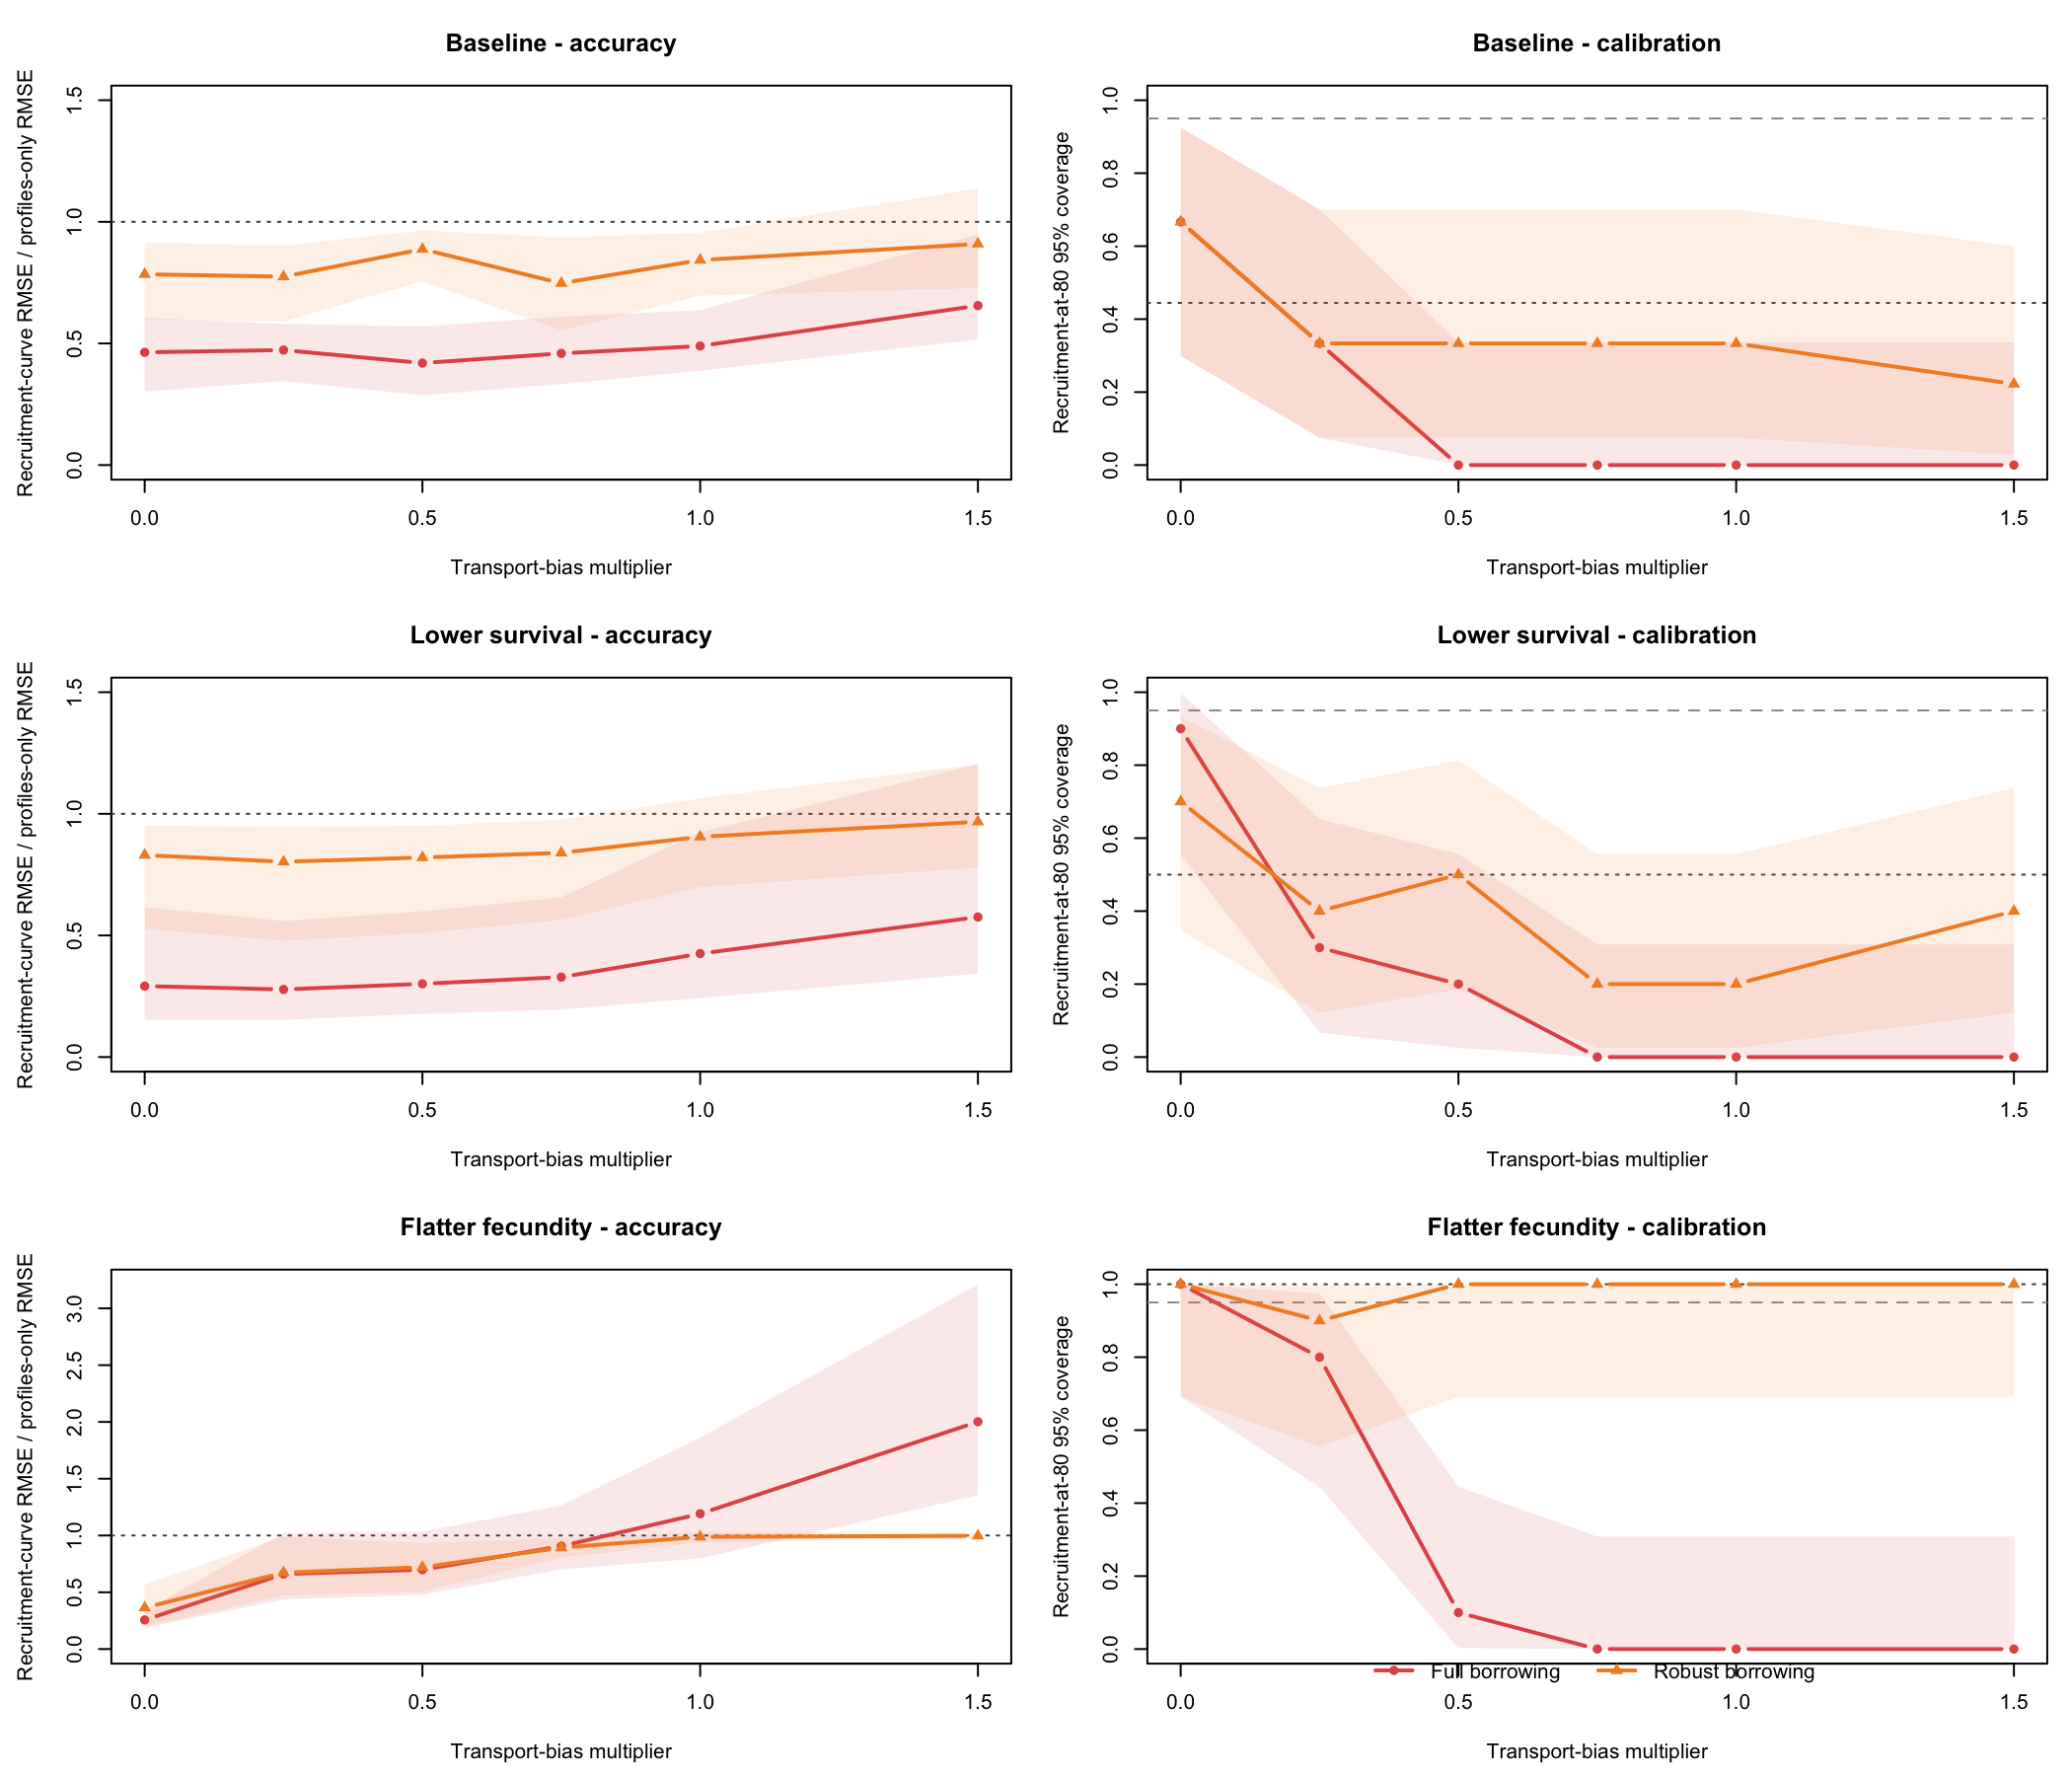
\includegraphics[width=\textwidth]{transportability_boundary/borrowing_safety_boundary.png}
\caption{Accuracy and calibration as transport bias increased. Horizontal
dotted lines show profiles-only performance; dashed lines show nominal 95\%
coverage. The safety of robust borrowing depended strongly on the generating
biology.}
\label{fig:safety-boundary}
\end{figure}

Using the conservative definition that the paired RMSE-ratio interval must
remain below one and coverage must not fall below profiles-only coverage, the
largest tested safe full-borrowing bias was zero for all three truths. The
largest tested safe robust-borrowing bias was zero under baseline biology,
0.50 under lower survival, and 0.75 under flatter fecundity. Because each
boundary point used only nine or ten paired datasets, these boundaries should
be treated as exploratory.

Robust borrowing rejected conflict only when profile dynamics were informative
about that conflict. Under flatter fecundity, posterior external-study weight
fell from approximately 0.91 with no bias to effectively zero by bias
multiplier 1.5. Under baseline and lower-survival biology, external-study
weight remained approximately 0.55--0.70 even under the largest tested bias
(Figure~\ref{fig:robust-weight}).

\begin{figure}[H]
\centering
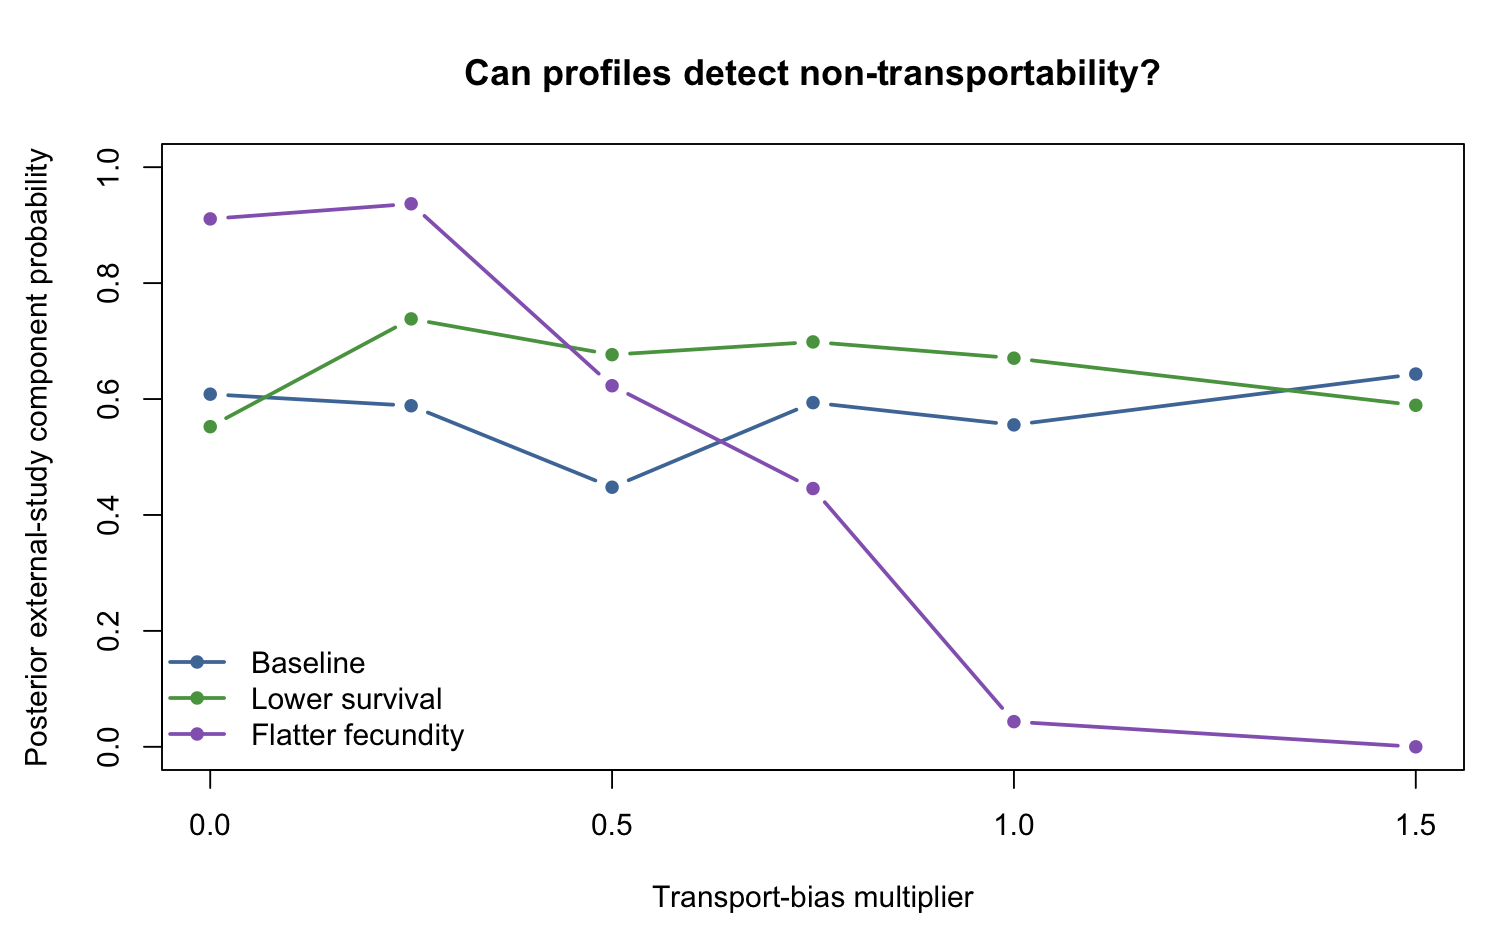
\includegraphics[width=0.82\textwidth]{transportability_boundary/robust_external_weight.png}
\caption{Mean posterior probability assigned to the external-study component
under robust borrowing. Profiles detected non-transportability under flatter
fecundity but not reliably under baseline or lower-survival biology.}
\label{fig:robust-weight}
\end{figure}

\subsection{Paired profile and individual-data benchmark}

All 1,200 paired-data fits completed, and 1,191 (99.25\%) had
positive-definite posterior Hessians. Approximation failures occurred only
under profile-only recovery: two Poisson and seven Gamma--Poisson fits.
Across datasets, the mean numbers observed were 1,499 fish in size profiles,
2,100 capture records, and 272 consecutive recaptures.

Capture--recapture directly and efficiently identified survival and growth
(Table~\ref{tab:paired-benchmark}). Its apparently perfect recruitment
coverage did not indicate recovery: recruitment and recruit-size parameters
contracted by less than 1\% from their weak priors, and the resulting
recruitment and population-growth intervals were extremely wide.

\begin{table}[H]
\centering
\caption{Paired-data benchmark across 200 simulated datasets. Entries are
empirical 95\% interval coverage / RMSE of posterior means.}
\label{tab:paired-benchmark}
\scriptsize
\setlength{\tabcolsep}{3pt}
\begin{tabular}{lcccc}
\toprule
Analysis & Survival at 80 mm & Growth increment at 80 mm &
Recruitment at 80 mm & Population growth\\
\midrule
Poisson profiles & 0.914 / 0.0267 & 0.889 / 0.904 & 0.495 / 0.143 & 0.737 / 0.0284\\
Gamma--Poisson profiles & 0.948 / 0.0257 & 0.876 / 0.905 & 0.570 / 0.148 & 0.772 / 0.0299\\
Capture--recapture & 0.970 / 0.0394 & 0.940 / 0.258 & 1.000 / 0.440 & 1.000 / 6.119\\
Poisson integrated & 0.795 / 0.0232 & 0.935 / 0.285 & 0.485 / 0.148 & 0.715 / 0.0258\\
Gamma--Poisson integrated & 0.850 / 0.0216 & 0.930 / 0.274 & 0.585 / 0.150 & 0.760 / 0.0264\\
Complete-history oracle & 0.960 / 0.0098 & 0.950 / 0.102 & 0.930 / 0.009 & 0.905 / 0.0140\\
\bottomrule
\end{tabular}
\end{table}

Integrated analyses improved survival point accuracy, but their intervals
became too narrow. Survival-at-80 coverage fell from 0.97 under
capture--recapture alone to 0.80 under Poisson integration and 0.85 under
Gamma--Poisson integration, despite lower RMSE. Recruitment coverage remained
poor. This pattern indicates that accurate individual transition information
anchored survival and growth while remaining discrepancies between observed
and deterministically projected profiles were absorbed by other demographic
parameters.

\begin{figure}[H]
\centering
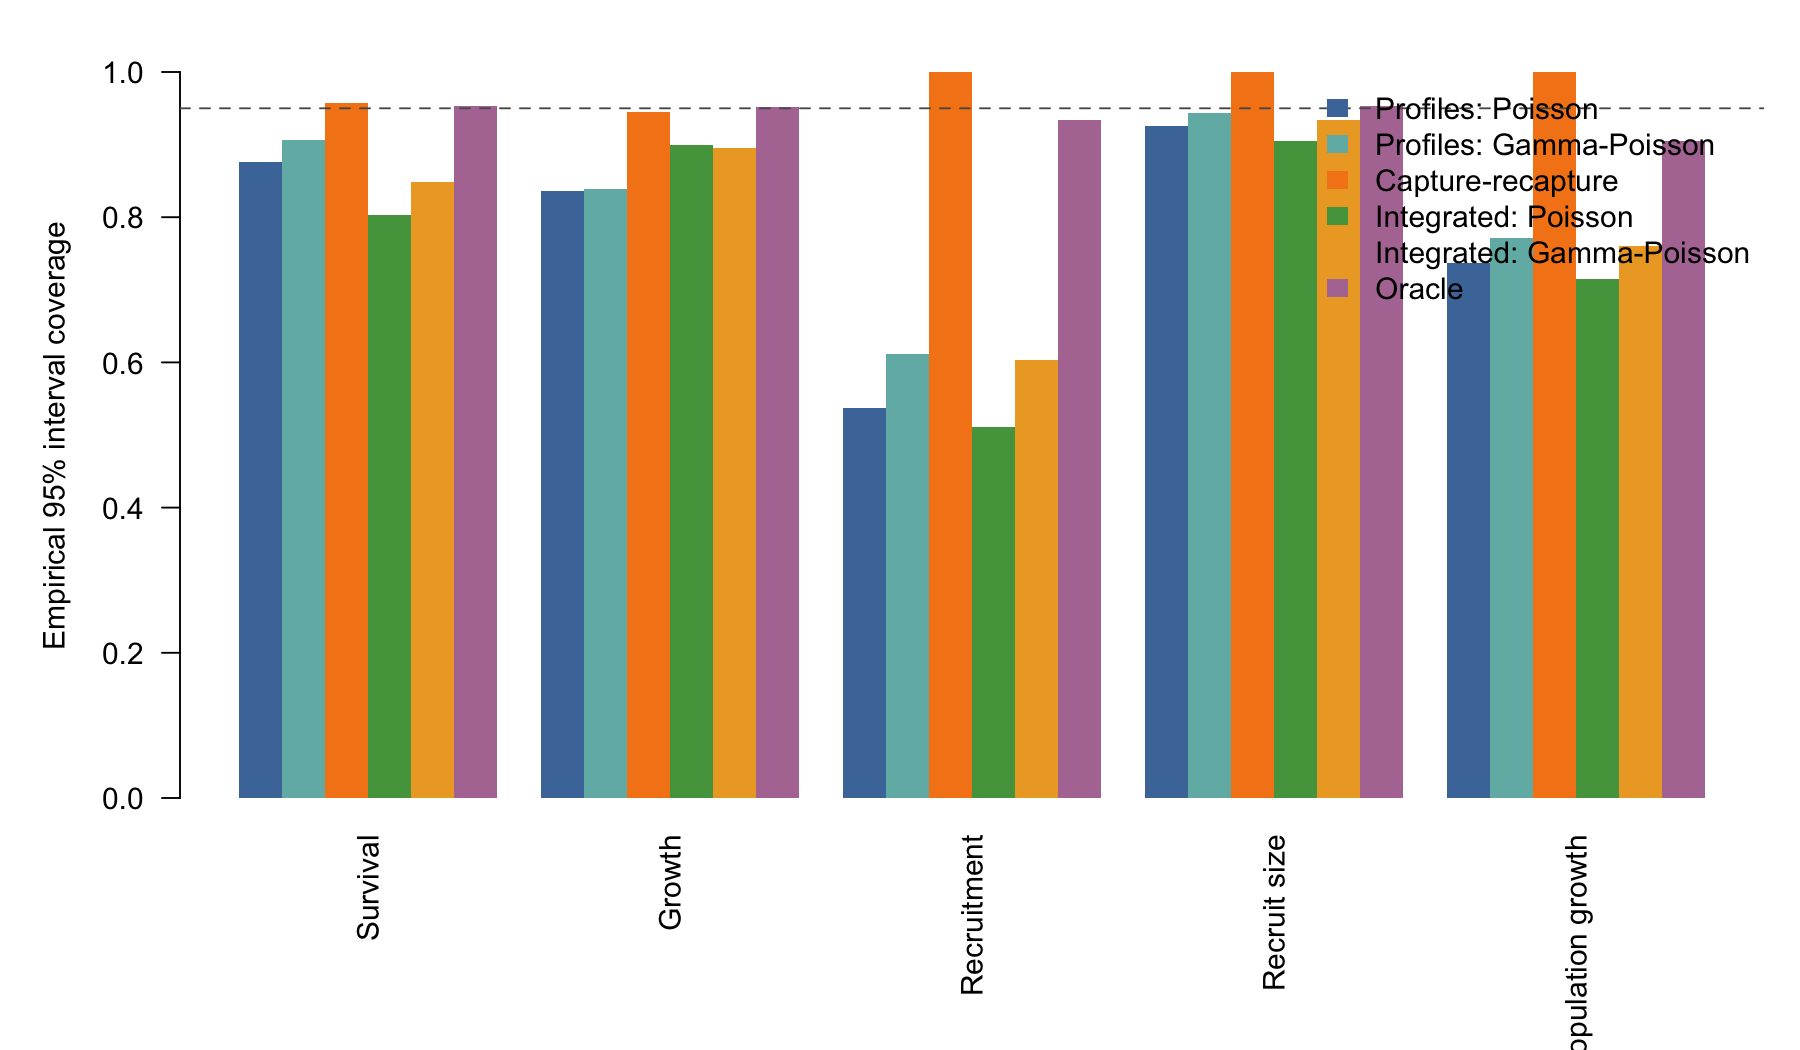
\includegraphics[width=\textwidth]{paired_benchmark/coverage_by_data_source.png}
\caption{Empirical interval coverage in the paired-data benchmark. Perfect
capture--recapture coverage for recruitment, recruit size, and population
growth reflects prior-dominated wide intervals rather than data-based
identification.}
\label{fig:paired-coverage}
\end{figure}

Gamma--Poisson overdispersion improved calibration but did not restore nominal
coverage. For example, it increased integrated recruitment coverage from 0.51
to 0.60 and integrated survival coverage from 0.80 to 0.85. Independent
bin-level overdispersion therefore absorbed some, but not all, of the
structured discrepancy generated by finite individual populations.

\end{document}
